% ============================================================
% FIGURE CAPTIONS FOR CELLULAR CHARGE TRAJECTORIES PAPER
% ============================================================

% PANEL 1: Partition Coordinates from Bounded Phase Space
\begin{figure*}[!htbp]
    \centering
    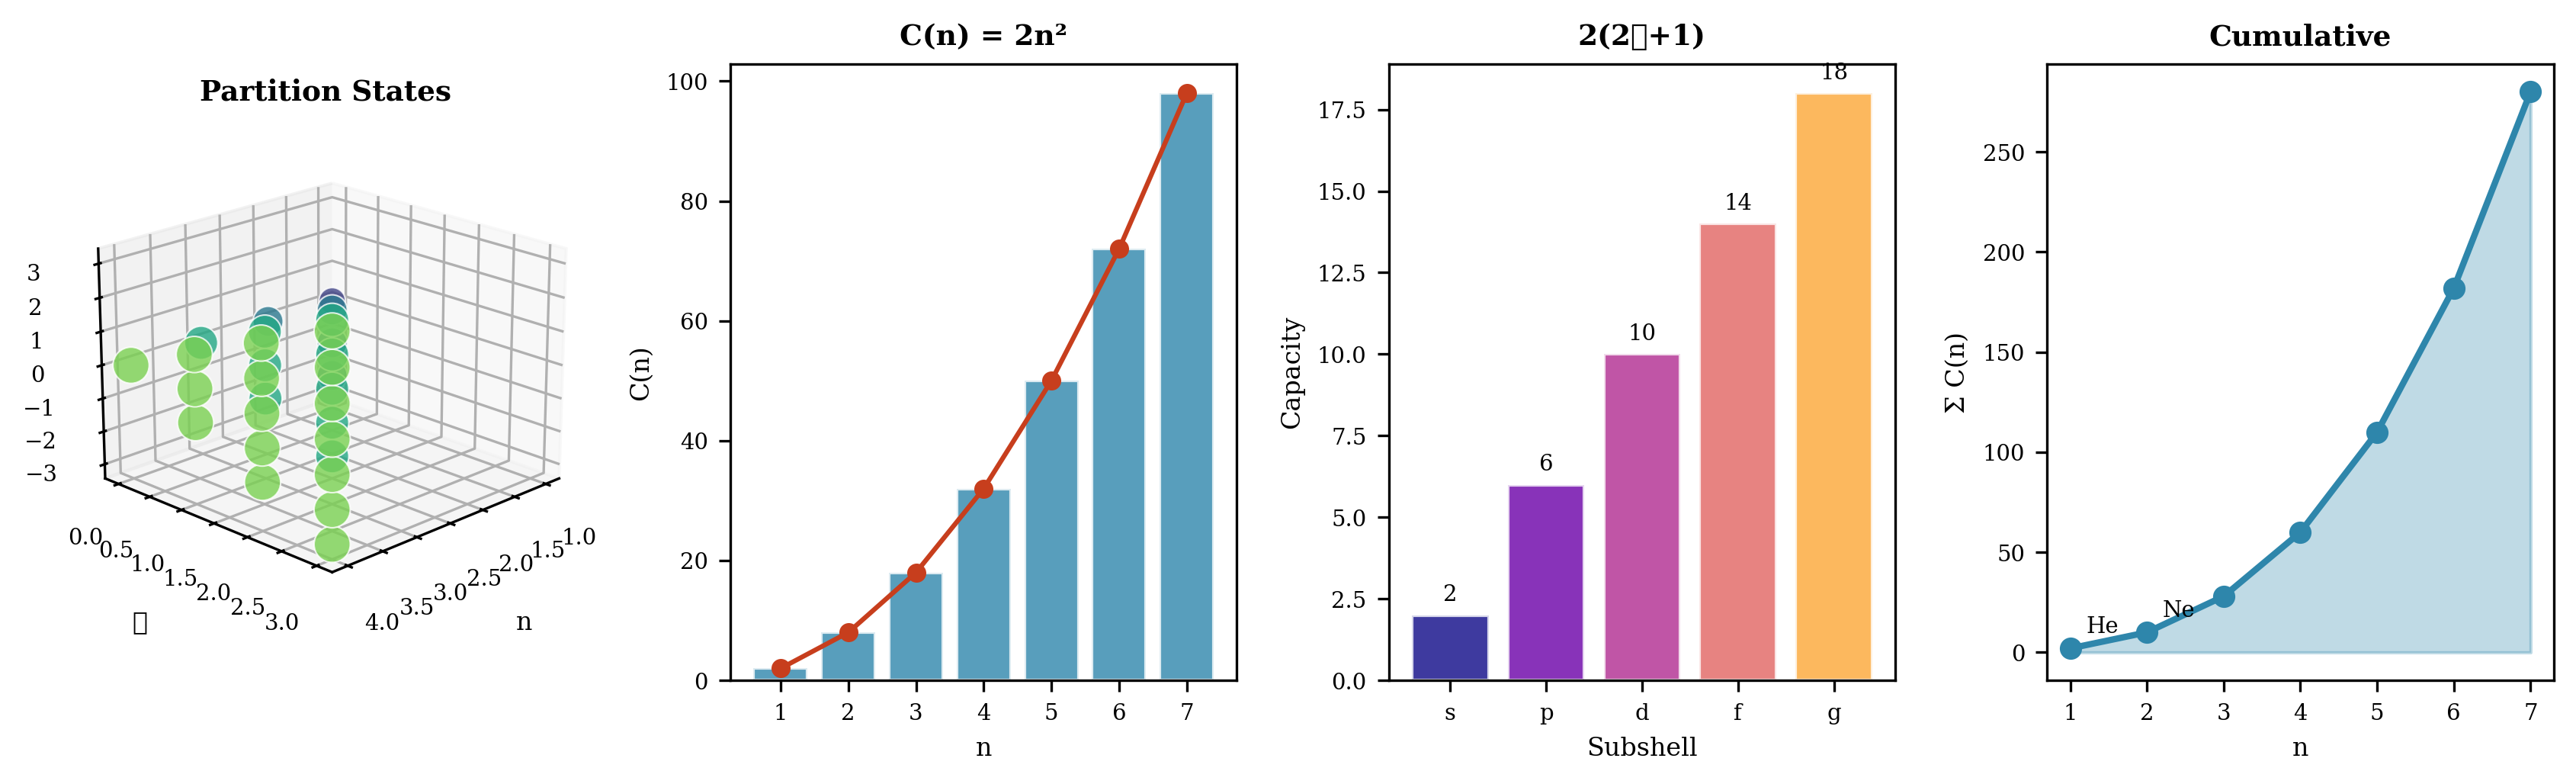
\includegraphics[width=\textwidth]{figures/panel1_partition.png}
    \caption{\textbf{Partition Coordinates from Bounded Phase Space: Derivation of categorical state structure.}
    (\textbf{A}) Three-dimensional visualization of partition states $(n, \ell, m)$ for principal quantum numbers $n = 1$ through $n = 4$. Each point represents a distinct categorical state in bounded phase space, with color gradient indicating nesting depth. States cluster at integer coordinates, demonstrating the discrete nature of partition space. The geometric constraints $\ell < n$ and $|m| \leq \ell$ are evident from the pyramidal distribution, with higher $n$ levels admitting more complex boundary topologies.
    (\textbf{B}) Capacity formula validation showing $C(n) = 2n^2$ for $n = 1$ to $7$. Blue bars indicate enumerated states per level; orange connected points confirm theoretical prediction. The quadratic scaling emerges from summing subshell contributions: $C(n) = 2\sum_{\ell=0}^{n-1}(2\ell + 1) = 2n^2$. This formula, derived purely from geometric constraints on bounded phase space, reproduces atomic electron shell capacities without invoking quantum mechanics.
    (\textbf{C}) Subshell capacity $C_\ell = 2(2\ell + 1)$ for s, p, d, f, g orbitals ($\ell = 0, 1, 2, 3, 4$). Color gradient indicates increasing boundary complexity. Values $\{2, 6, 10, 14, 18\}$ match spectroscopic observations, confirming that orbital multiplicity follows from the constraint $m \in \{-\ell, \ldots, +\ell\}$ combined with spin degeneracy $s = \pm 1/2$.
    (\textbf{D}) Cumulative state count $\sum_{k=1}^{n} C(k)$ showing total accessible states up to principal quantum number $n$. Shaded region indicates filled phase space volume. The sequence $\{2, 10, 28, 60, 110, \ldots\}$ determines periodic table structure, with noble gas configurations occurring at completed shells.}
    \label{fig:partition}
\end{figure*}

% PANEL 2: Selection Rules from Boundary Continuity
\begin{figure*}[!htbp]
    \centering
    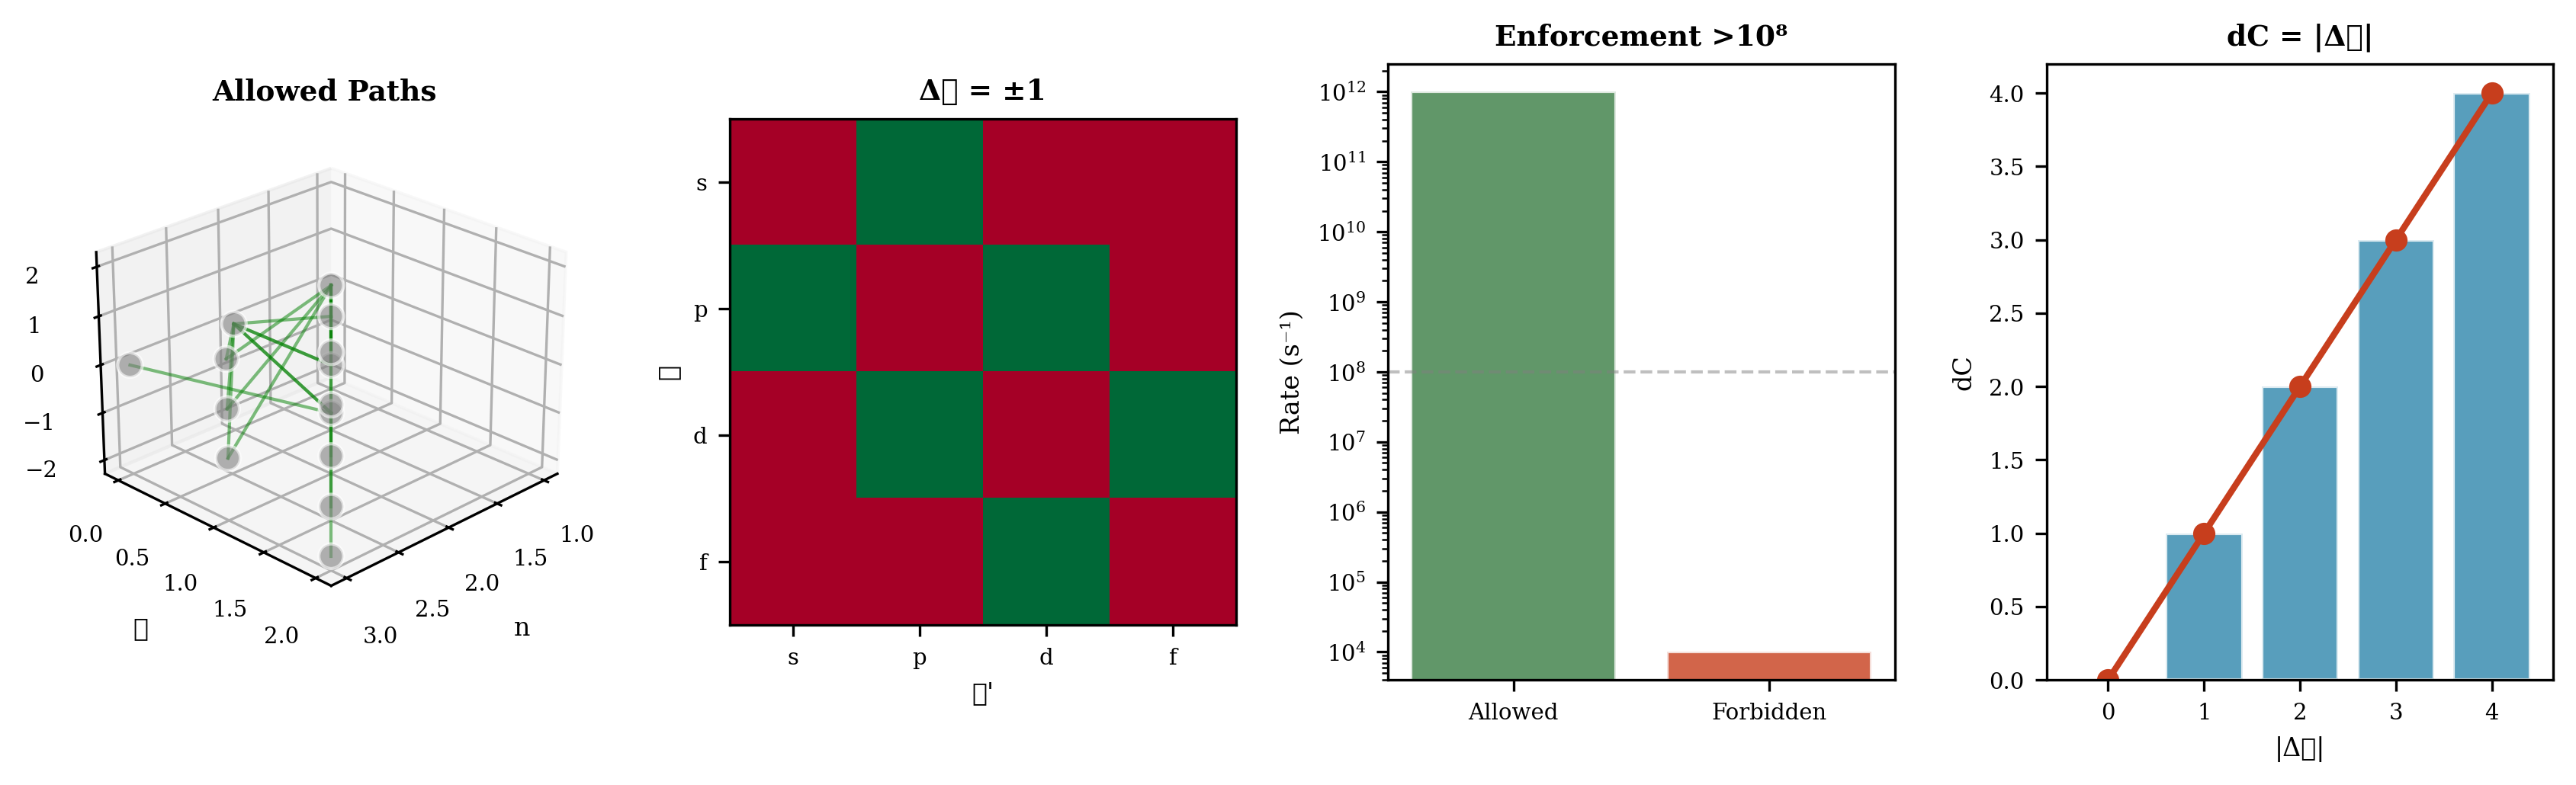
\includegraphics[width=\textwidth]{figures/panel2_selection.png}
    \caption{\textbf{Selection Rules from Boundary Continuity: Constraints on categorical state transitions.}
    (\textbf{A}) Three-dimensional transition pathways through $(n, \ell, m)$ partition space. Gray spheres mark categorical states; green lines indicate allowed transitions satisfying $\Delta\ell = \pm 1$ and $|\Delta m| \leq 1$. Forbidden transitions (not shown) would require discontinuous boundary deformation. The pathway topology constrains electron dynamics: transitions must traverse adjacent complexity levels, preventing direct jumps between distant states.
    (\textbf{B}) Selection rule matrix for angular momentum transitions. Green cells indicate allowed transitions between subshells (s$\leftrightarrow$p, p$\leftrightarrow$d, d$\leftrightarrow$f); red cells indicate forbidden transitions (s$\leftrightarrow$d, s$\leftrightarrow$f, p$\leftrightarrow$f). The rule $\Delta\ell = \pm 1$ emerges from the requirement that boundary complexity changes continuously---a spherical boundary cannot directly become a four-lobed shape without passing through two-lobed intermediate.
    (\textbf{C}) Enforcement ratio comparing allowed and forbidden transition rates. Allowed transitions proceed at $\Gamma_{\text{allowed}} \sim 10^{12}$~s$^{-1}$ (picosecond timescale); forbidden transitions are suppressed to $\Gamma_{\text{forbidden}} \sim 10^{4}$~s$^{-1}$. The ratio exceeds $10^8$, rendering forbidden pathways effectively inaccessible on relevant timescales. Gray dashed line marks the $10^8$ threshold.
    (\textbf{D}) Categorical distance $d_{\text{C}} = |\Delta\ell|$ as function of angular momentum change. Each unit of categorical distance requires one allowed transition, determining minimum transition time $\tau \geq d_{\text{C}} \cdot \tau_{\text{step}}$. Fast catalytic processes require $d_{\text{C}} = 1$; slower multi-step reactions have $d_{\text{C}} > 1$.}
    \label{fig:selection}
\end{figure*}

% PANEL 3: Phase-Lock Dynamics from Coupled Oscillators
\begin{figure*}[!htbp]
    \centering
    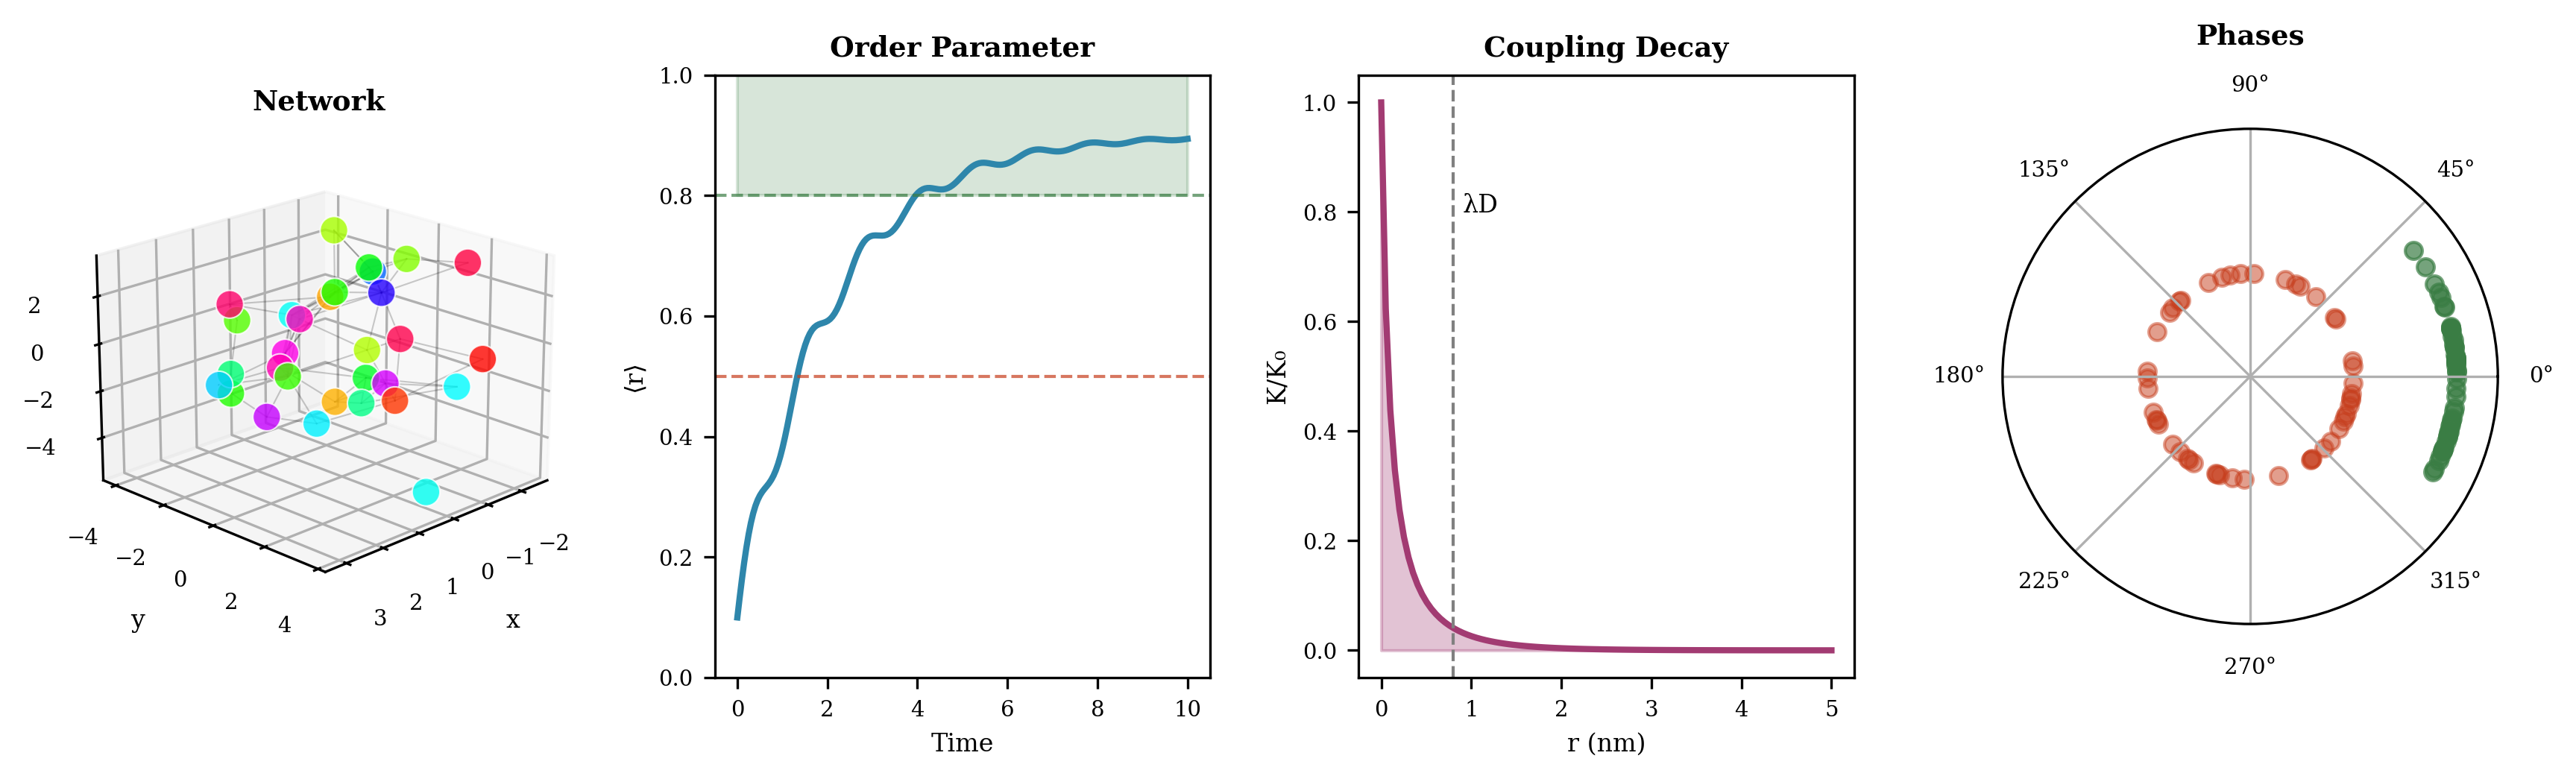
\includegraphics[width=\textwidth]{figures/panel3_phaselock.png}
    \caption{\textbf{Phase-Lock Dynamics from Coupled Oscillators: Synchronization in bounded charge systems.}
    (\textbf{A}) Three-dimensional oscillator network with nodes colored by phase $\phi_i \in [0, 2\pi)$. Black lines indicate coupling connections between oscillators separated by less than the cutoff distance. Phase coherence is visible as color clustering---synchronized oscillators share similar hues. The network topology determines synchronization dynamics through the Kuramoto equation $d\phi_i/dt = \omega_i + \sum_j K_{ij}\sin(\phi_j - \phi_i)$.
    (\textbf{B}) Order parameter $\langle r \rangle = |N^{-1}\sum_j e^{i\phi_j}|$ evolution during synchronization transition. Starting from disorder ($\langle r \rangle \approx 0.1$), the system synchronizes to $\langle r \rangle > 0.8$ over characteristic time $\tau_{\text{sync}}$. Green dashed line marks the stability threshold $\langle r \rangle = 0.8$ for native structure; red dashed line marks the instability threshold $\langle r \rangle = 0.5$ below which structures misfold.
    (\textbf{C}) Coupling strength decay $K(r)/K_0 = e^{-r/\lambda_{\text{D}}}/r$ as function of distance in electrolyte. The Debye screening length $\lambda_{\text{D}} \approx 0.8$~nm (gray dashed line) sets the characteristic interaction range. Coupling falls exponentially beyond $\lambda_{\text{D}}$, limiting phase coherence to nanometer-scale domains. This screening underlies the locality of charge dynamics in ionic solution.
    (\textbf{D}) Polar distribution of oscillator phases showing synchronized (outer ring, green, $\langle r \rangle > 0.8$) versus disordered (inner ring, red, $\langle r \rangle \approx 0$) configurations. Synchronized phases cluster near $\phi = 0$; disordered phases distribute uniformly around the circle. The native structure corresponds to the global minimum of phase variance across the oscillator network.}
    \label{fig:phaselock}
\end{figure*}

% PANEL 4: Four-State Partition Operators from Electron Transport
\begin{figure*}[!htbp]
    \centering
    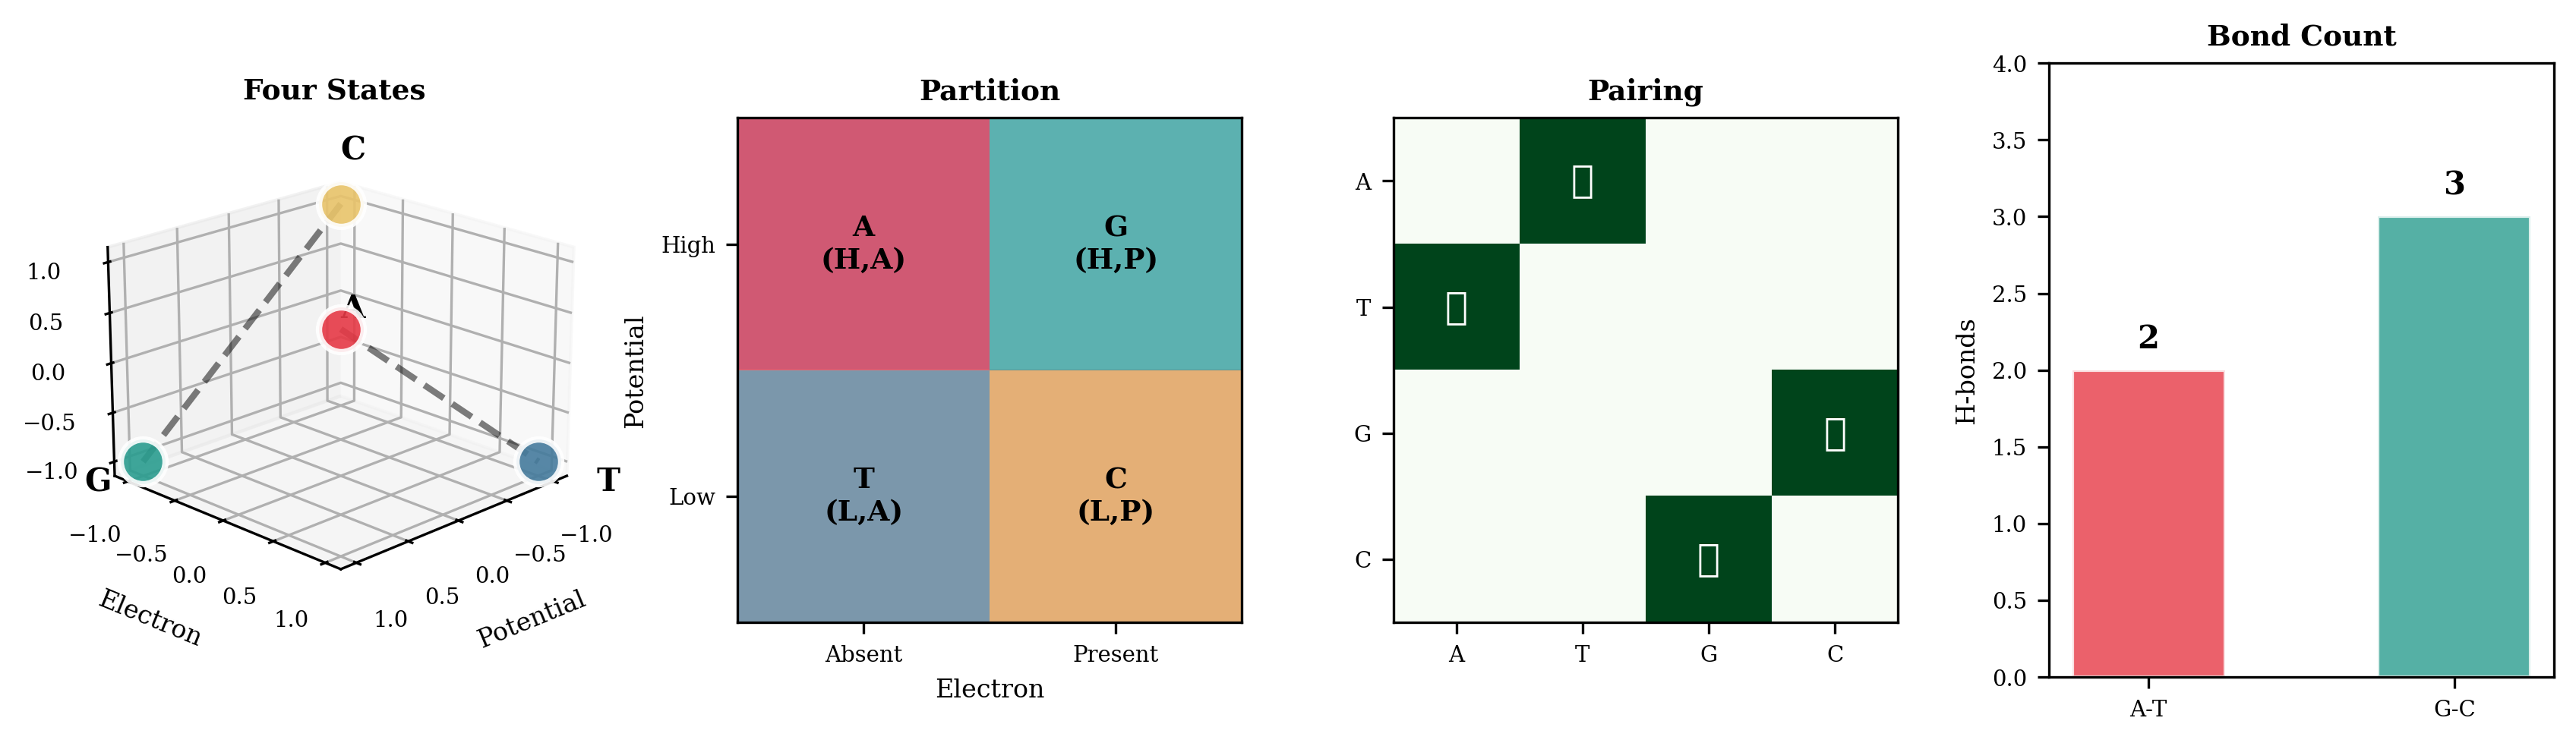
\includegraphics[width=\textwidth]{figures/panel4_fourstate.png}
    \caption{\textbf{Four-State Partition Operators from Electron Transport: Nucleotide correspondence.}
    (\textbf{A}) Three-dimensional representation of four categorical states generated by electron transport partitioning. States occupy vertices of a tetrahedron-like configuration in partition space, with complementary pairs (A-T, G-C) connected by dashed lines. The four states arise from two binary partitions: $\mathcal{P}_1 = \{\text{high potential}, \text{low potential}\}$ and $\mathcal{P}_2 = \{\text{electron present}, \text{electron absent}\}$, yielding $2 \times 2 = 4$ combined states.
    (\textbf{B}) Partition diagram mapping four states to nucleotide bases. Adenine (A) corresponds to (High, Absent); Thymine (T) to (Low, Absent); Guanine (G) to (High, Present); Cytosine (C) to (Low, Present). Color coding matches standard nucleotide representations. This correspondence emerges from the charge stabilization requirements of partition operators, not from arbitrary assignment.
    (\textbf{C}) Complementarity matrix showing Watson-Crick base pairing as partition symmetry. Checkmarks indicate allowed pairs: A pairs with T (potential inversion, electron state preserved), G pairs with C (potential inversion, electron state preserved). Complementarity enforces local charge neutralization---high-potential states pair with low-potential states, balancing the electrostatic environment across each base pair.
    (\textbf{D}) Hydrogen bond count for complementary pairs: A-T pairs have 2 H-bonds; G-C pairs have 3 H-bonds. The additional H-bond in G-C contributes $\sim$1~kcal/mol extra stability. Total H-bonds in the human genome: $N_{\text{H-bond}} = 2N_{\text{AT}} + 3N_{\text{GC}} \approx 7.5 \times 10^9$, establishing the scale of the phase-lock oscillator network.}
    \label{fig:fourstate}
\end{figure*}

% PANEL 5: Charge Stabilization Architecture
\begin{figure*}[!htbp]
    \centering
    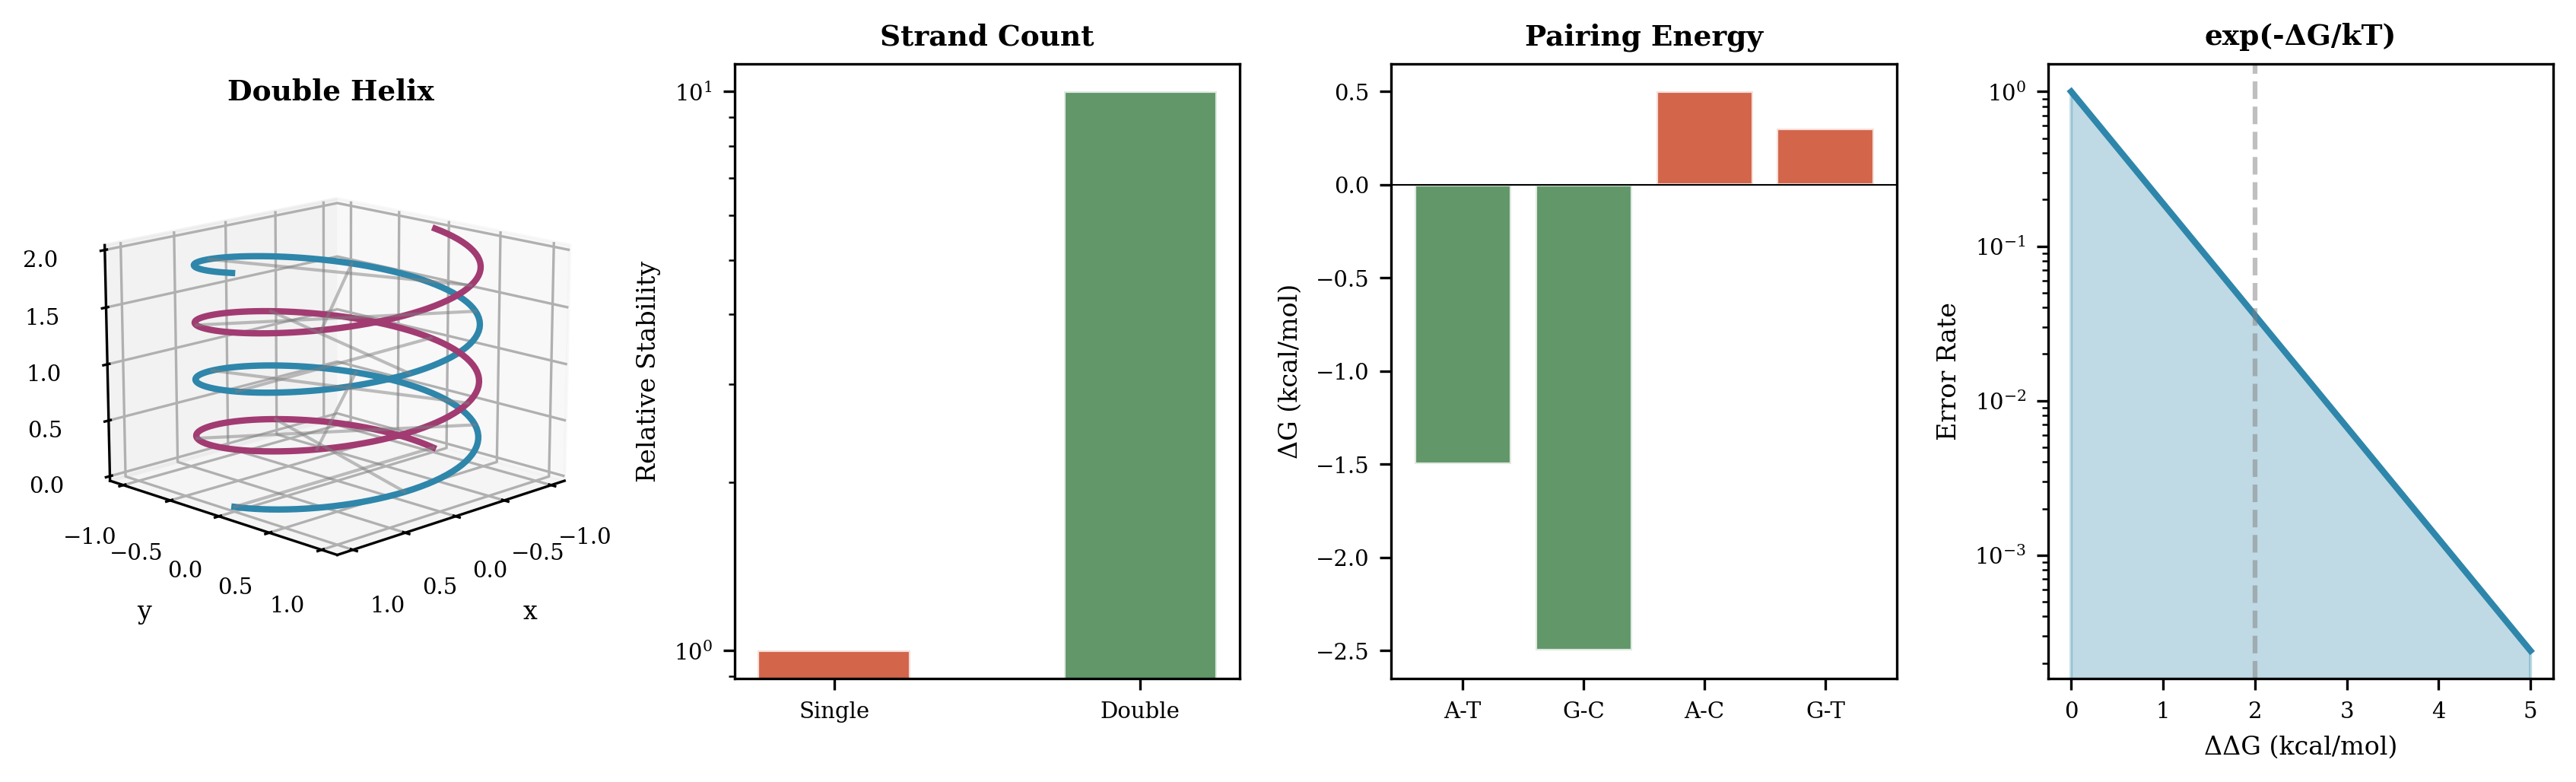
\includegraphics[width=\textwidth]{figures/panel5_architecture.png}
    \caption{\textbf{Charge Stabilization Architecture: Double-strand requirement from partition stability.}
    (\textbf{A}) Three-dimensional double helix structure showing antiparallel strand orientation. Blue strand runs 5'$\to$3'; purple strand runs 3'$\to$5'. Gray rungs represent base pairs connecting the strands. The helical geometry with $\sim$10.5 bp per turn maximizes base stacking interactions while maintaining Watson-Crick hydrogen bonding geometry. This architecture emerges as the minimum structure providing stable partition operator storage.
    (\textbf{B}) Relative stability comparison between single-stranded and double-stranded configurations (log scale). Double-stranded architecture provides $\sim$10-fold greater thermal stability against partition state corruption. The energy difference $\Delta G_{\text{ds}} - \Delta G_{\text{ss}} \approx 1$--3~kcal/mol per base pair exceeds $k_{\text{B}}T$ at physiological temperature, ensuring partition fidelity.
    (\textbf{C}) Base pairing energies $\Delta G$ (kcal/mol) for matched (A-T, G-C) and mismatched (A-C, G-T) pairs. Matched pairs have negative $\Delta G$ (favorable); mismatched pairs have positive $\Delta G$ (unfavorable). The energy penalty $\Delta\Delta G_{\text{mismatch}} \approx 2$--4~kcal/mol drives proofreading and mismatch repair mechanisms, maintaining partition integrity during replication.
    (\textbf{D}) Error rate as function of energy penalty, following Boltzmann statistics: $P_{\text{error}} \sim e^{-\Delta\Delta G/k_{\text{B}}T}$. Gray dashed line marks typical mismatch penalty $\sim$2~kcal/mol, yielding intrinsic error rate $\sim$10$^{-2}$--10$^{-4}$. Combined with proofreading and repair, achieved fidelity reaches $10^{-9}$--10$^{-10}$ per base pair.}
    \label{fig:architecture}
\end{figure*}

% PANEL 6: Capacitive Properties of Nucleic Acid Polymers
\begin{figure*}[!htbp]
    \centering
    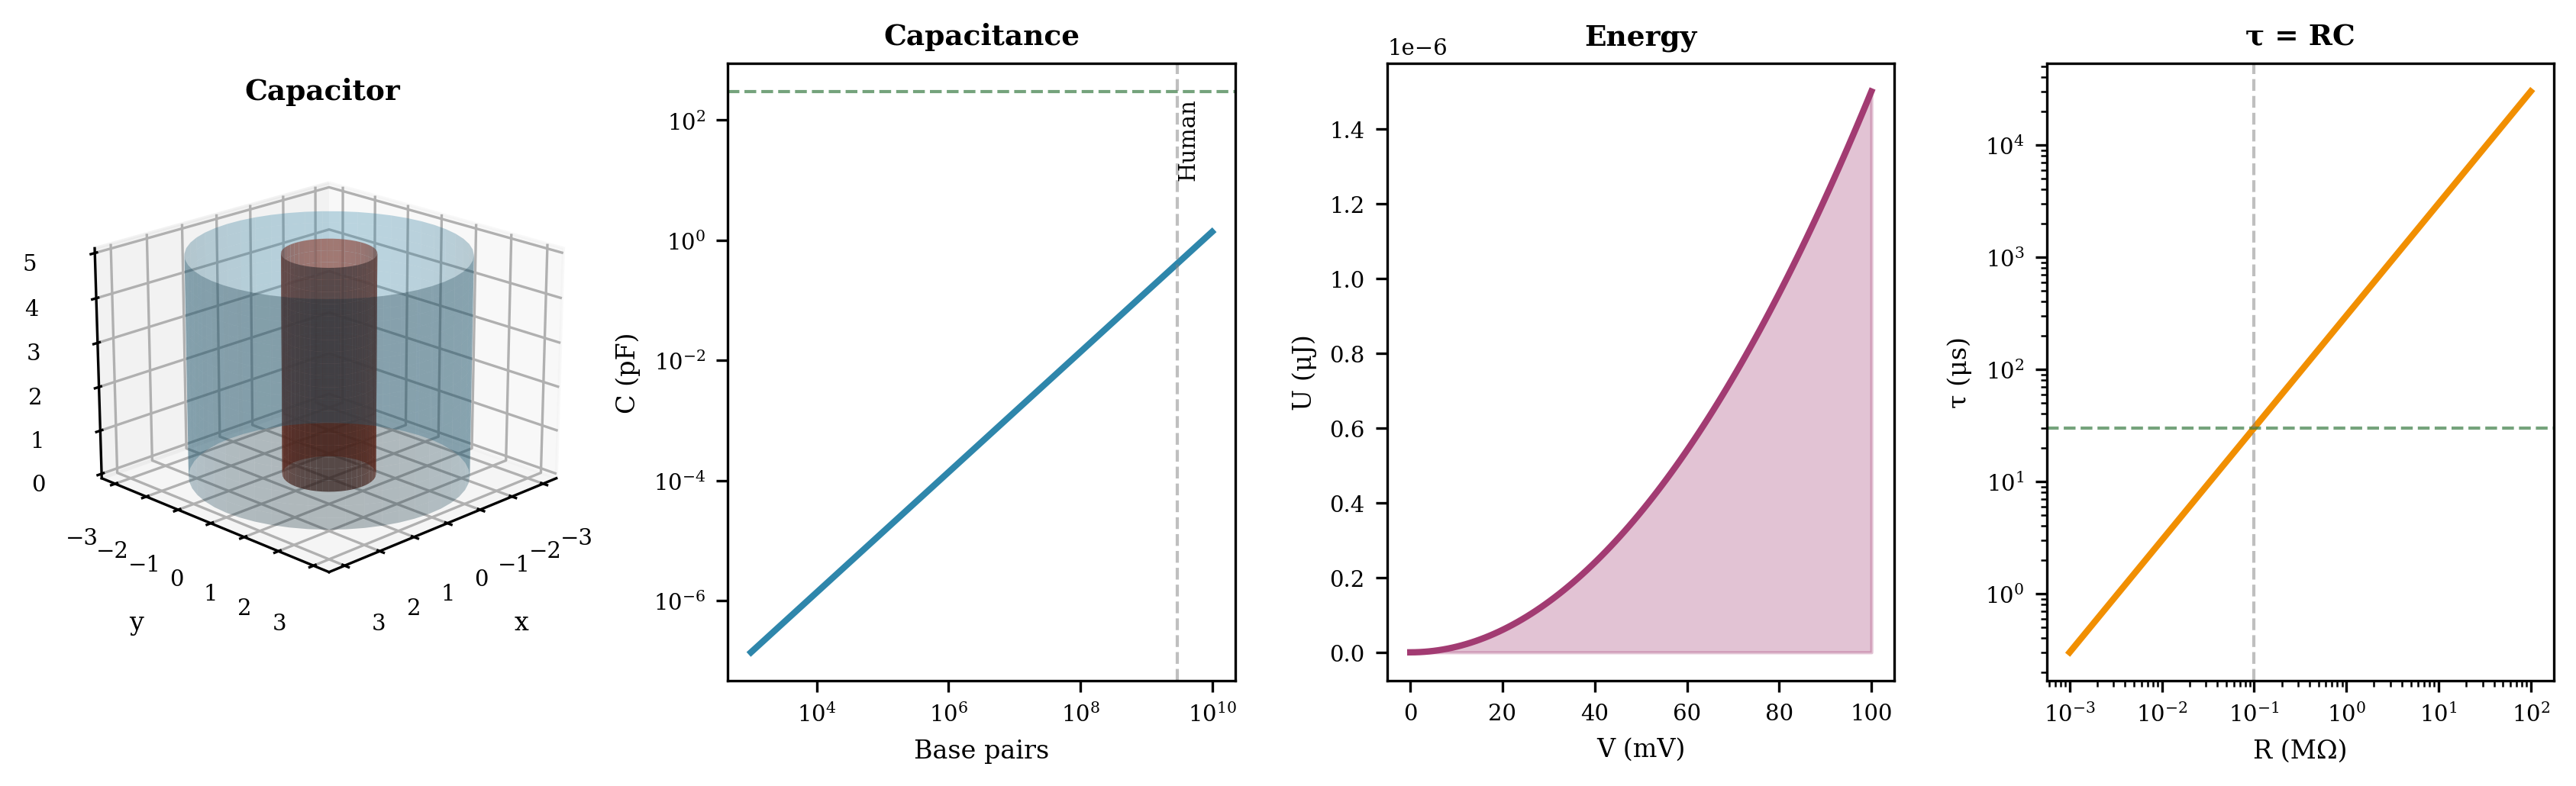
\includegraphics[width=\textwidth]{figures/panel6_capacitance.png}
    \caption{\textbf{Capacitive Properties of Nucleic Acid Polymers: Charge storage in genomic DNA.}
    (\textbf{A}) Three-dimensional cylindrical capacitor model of DNA in ionic solution. Inner cylinder (red, radius $a \approx 1$~nm) represents the phosphate backbone with fixed negative charge; outer cylinder (blue, transparent, radius $b \approx 3$~nm) represents the counterion cloud. The aqueous dielectric ($\varepsilon_r \approx 80$) separates the electrodes, establishing capacitor geometry $C = 2\pi\varepsilon_0\varepsilon_r L/\ln(b/a)$.
    (\textbf{B}) Capacitance scaling with genome size (base pairs) on log-log axes. Blue curve shows theoretical prediction accounting for chromatin compaction; green dashed line marks $C = 300$~pF corresponding to human genome ($3 \times 10^9$~bp, gray dashed vertical). The scaling follows $C \propto N$ for extended DNA, modified by compaction ratio $\sim$10$^4$ in chromatin.
    (\textbf{C}) Electrostatic energy storage $U = \frac{1}{2}CV^2$ as function of voltage (mV) for $C = 300$~pF. At membrane potential $V \sim 100$~mV, stored energy reaches $\sim$1.5~$\mu$J, exceeding the cellular ATP pool by four orders of magnitude. This energy maintains electrostatic organization rather than powering biochemical work.
    (\textbf{D}) RC time constant $\tau = RC$ as function of resistance (M$\Omega$) for $C = 300$~pF. Green dashed line marks $\tau = 30$~$\mu$s corresponding to estimated nuclear resistance $R \sim 0.1$~M$\Omega$. This timescale matches fast cellular signaling, suggesting coupling between genomic charge dynamics and physiological processes.}
    \label{fig:capacitance}
\end{figure*}

% PANEL 7: Polymerase Catalysis as Capacitor-Mediated Charge Transfer
\begin{figure*}[!htbp]
    \centering
    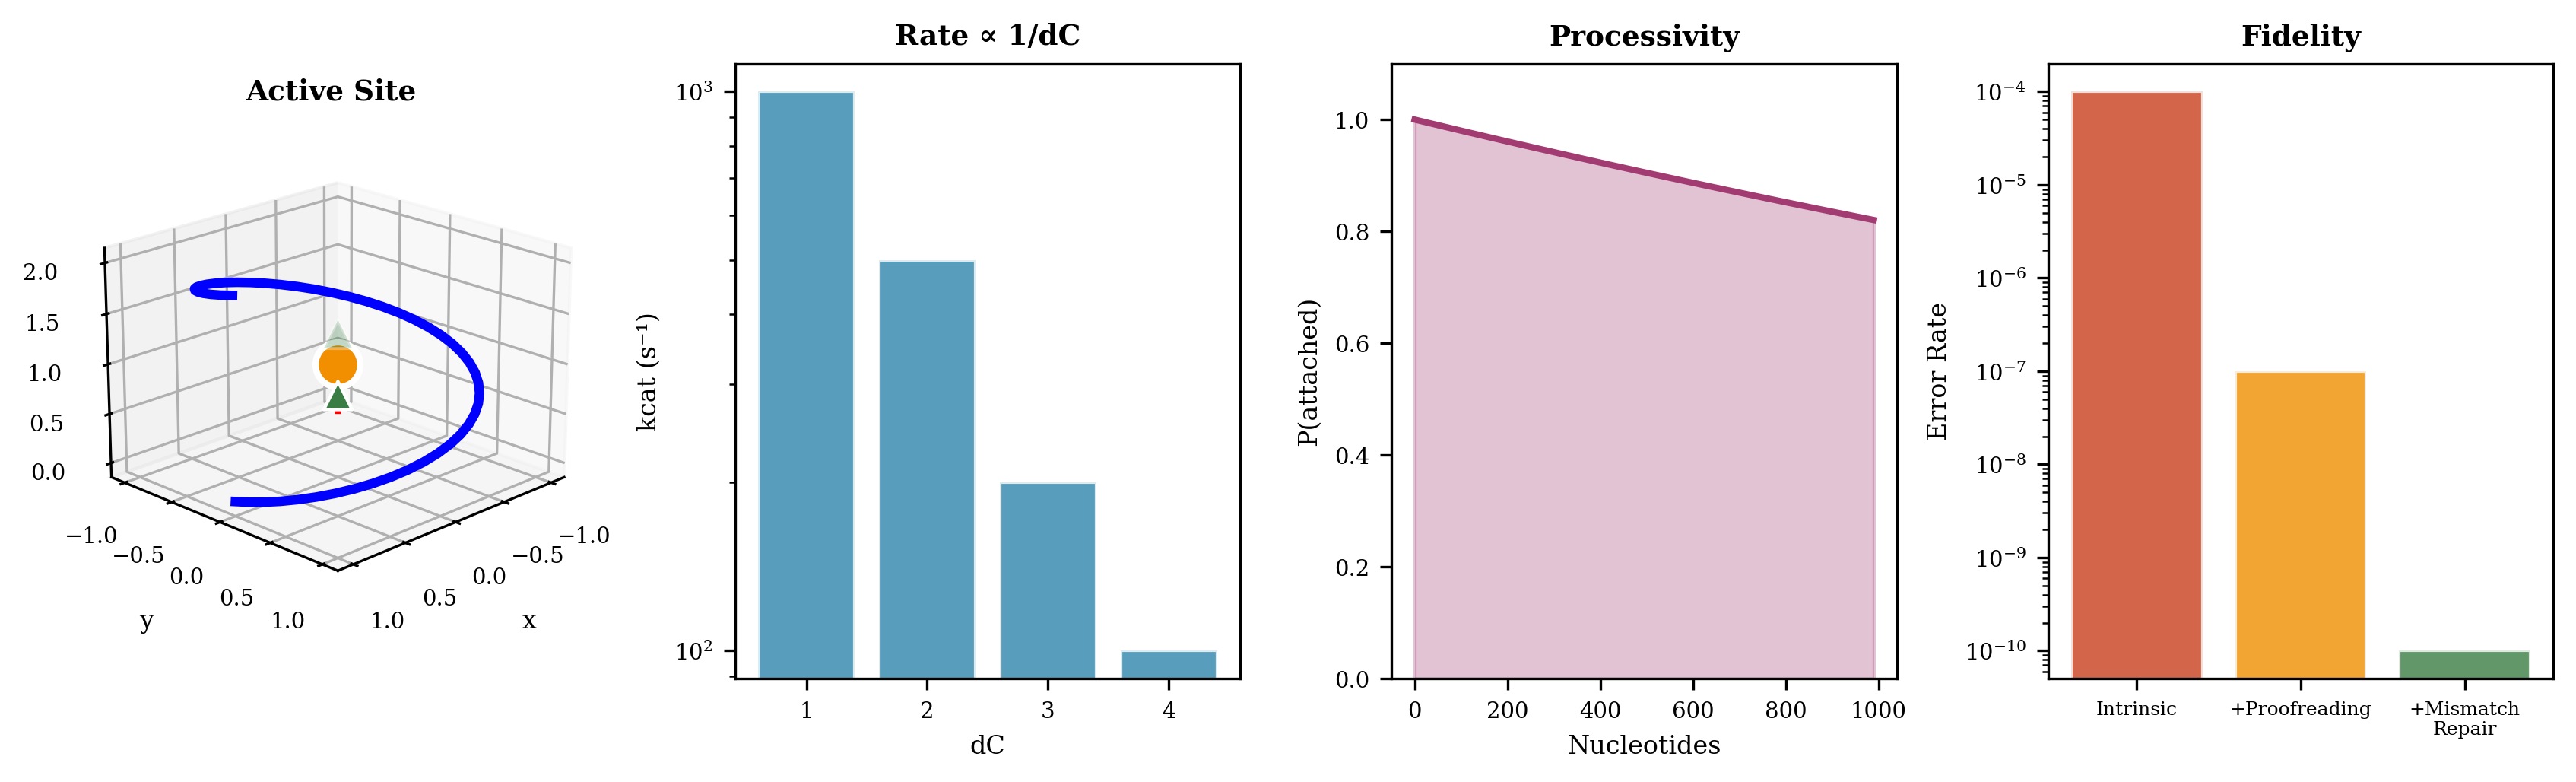
\includegraphics[width=\textwidth]{figures/panel7_polymerase.png}
    \caption{\textbf{Polymerase Catalysis as Capacitor-Mediated Charge Transfer: Nucleotide incorporation mechanism.}
    (\textbf{A}) Three-dimensional active site schematic showing template strand (blue helix), incoming dNTP (orange sphere), and catalytic Mg$^{2+}$ ions (green triangles). Red arrow indicates incorporation direction (5'$\to$3'). The two-metal-ion mechanism coordinates triphosphate hydrolysis with phosphodiester bond formation, transferring one net negative charge to the growing strand per incorporation event.
    (\textbf{B}) Turnover rate $k_{\text{cat}}$ (s$^{-1}$, log scale) as function of categorical distance $d_{\text{C}}$. Each increment in $d_{\text{C}}$ corresponds to an additional partition boundary crossing, adding $\tau_{\text{step}} \approx 1$~ps to minimum reaction time. DNA polymerase achieves $d_{\text{C}} = 1$ (single transition), enabling rates $\sim$10$^3$~s$^{-1}$ limited by dNTP binding rather than chemical catalysis.
    (\textbf{C}) Processivity curve showing probability of remaining attached as function of nucleotides incorporated. High processivity ($>$10$^4$ nt per binding event) arises from capacitive coupling: each incorporation adds charge to the DNA reservoir, strengthening electrostatic association. The exponential decay reflects the dissociation barrier $\Delta G_{\text{dissoc}} \approx 5$~kcal/mol.
    (\textbf{D}) Fidelity enhancement through successive mechanisms. Intrinsic selectivity yields error rate $\sim$10$^{-4}$; proofreading (3'$\to$5' exonuclease) reduces to $\sim$10$^{-7}$; mismatch repair achieves $\sim$10$^{-10}$. Each mechanism exploits charge mismatch detection---incorrect bases disrupt local electrostatic balance, triggering removal.}
    \label{fig:polymerase}
\end{figure*}

% PANEL 8: Cellular Charge Architecture
\begin{figure*}[!htbp]
    \centering
    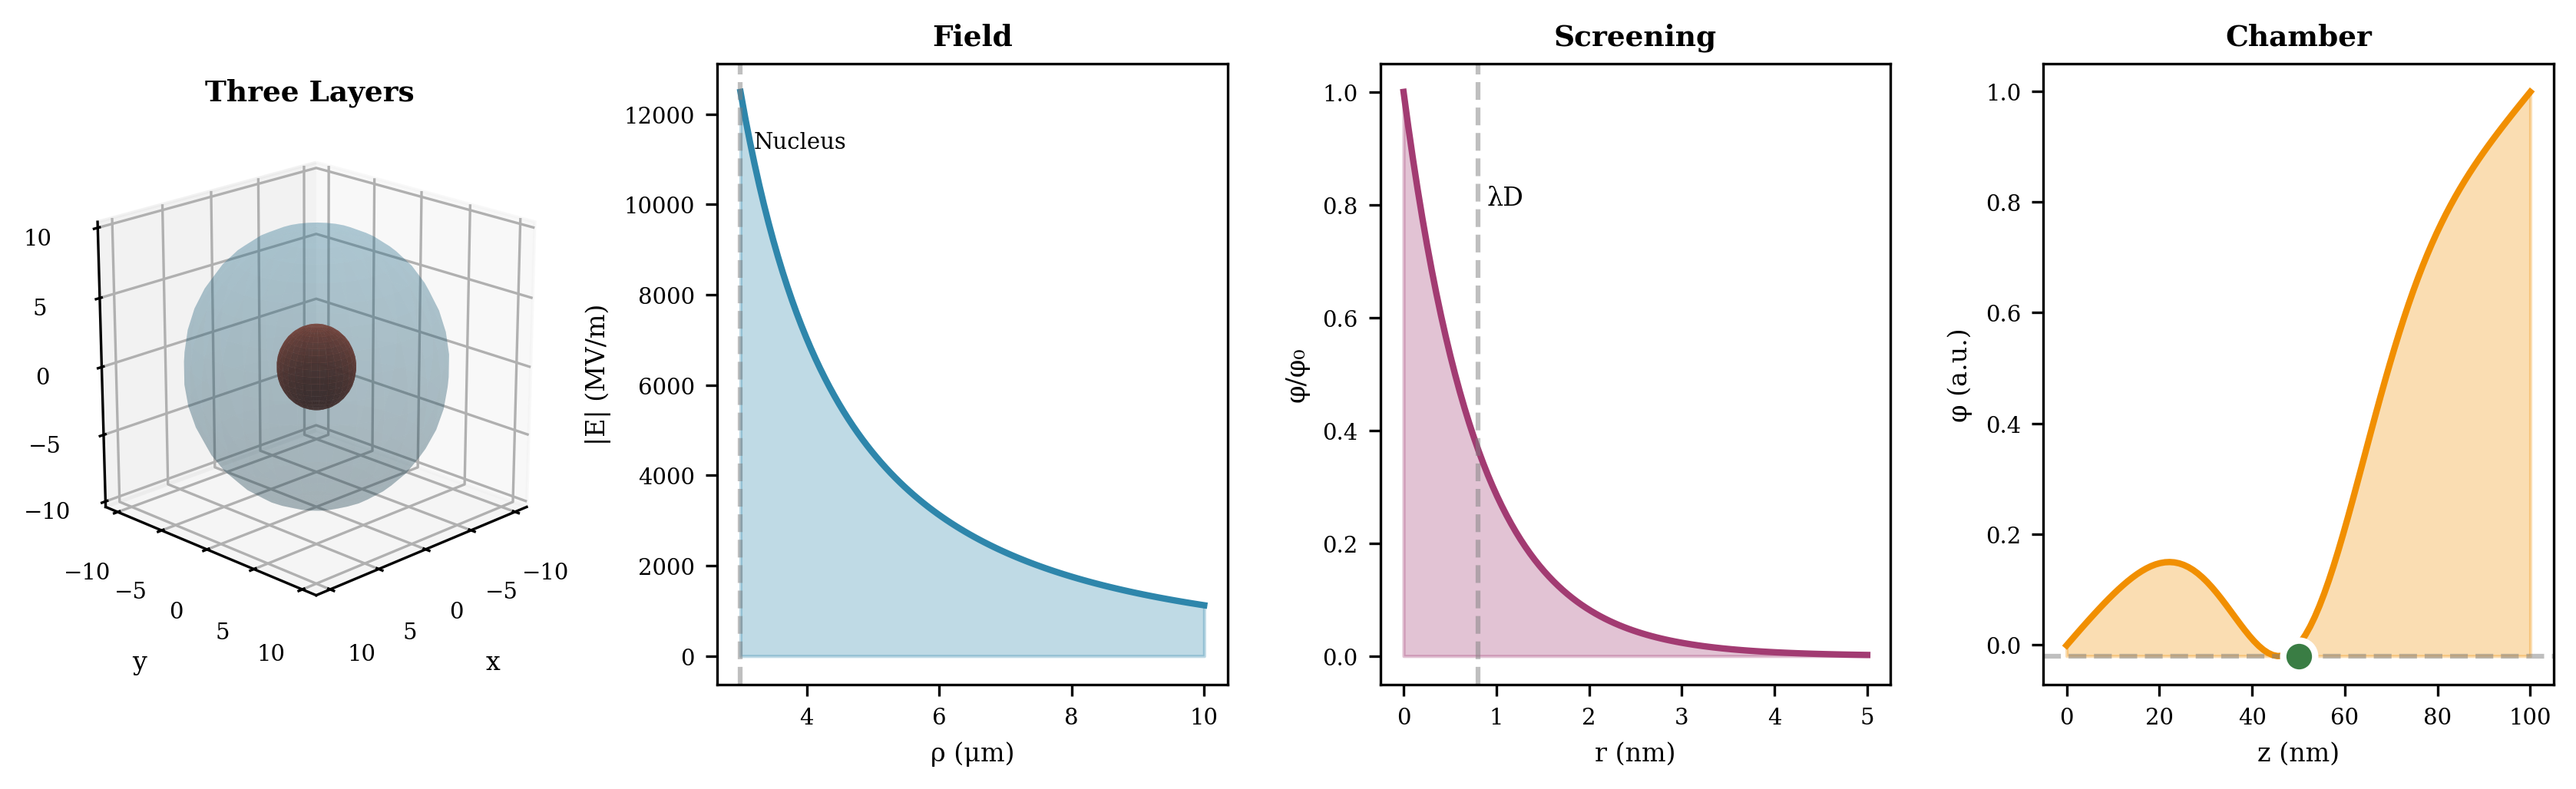
\includegraphics[width=\textwidth]{figures/panel8_cellular.png}
    \caption{\textbf{Cellular Charge Architecture: Three-layer electrostatic organization.}
    (\textbf{A}) Three-dimensional representation of the three-layer cellular capacitor. Inner sphere (red, $r \approx 3$~$\mu$m) represents the nucleus containing genomic charge $Q_{\text{gen}} \approx -1$~nC; outer sphere (blue, transparent, $R \approx 10$~$\mu$m) represents the plasma membrane with dynamic surface charge $Q_{\text{mem}}$. The cytoplasmic electrolyte between layers contains mobile counterions maintaining approximate electroneutrality.
    (\textbf{B}) Electric field magnitude $|\mathbf{E}|$ (MV/m) as function of radial distance $\rho$ ($\mu$m) from cell center. Field strength peaks at the nuclear envelope ($\rho = 3$~$\mu$m, gray dashed line) and decays as $1/\rho^2$ toward the membrane. Unscreened field reaches $\sim$1~MV/m at the nuclear surface---sufficient to influence molecular orientation and transport.
    (\textbf{C}) Debye-H\"{u}ckel screening of electrostatic potential $\phi/\phi_0 = e^{-r/\lambda_{\text{D}}}$ as function of distance $r$ (nm) from a charged surface. Screening length $\lambda_{\text{D}} \approx 0.8$~nm (gray dashed line) at physiological ionic strength. Beyond $\sim$3~nm, electrostatic interactions are effectively screened, limiting direct charge coupling to nanometer scales.
    (\textbf{D}) Electrostatic chamber formation from superposition of genomic and membrane fields. Plot shows total potential $\phi$ (arbitrary units) versus distance $z$ (nm) from membrane. The potential minimum (green circle) at $z^* \approx 50$~nm defines the chamber location where molecules are electrostatically confined. Chamber volume $V_{\text{ch}} \sim 10^{-22}$~m$^3$ enables reaction localization without diffusive search.}
    \label{fig:cellular}
\end{figure*}
